% -------------------------------------------------------------------------
% LaTeX Vorlage fuer wissenschaftliche Arbeiten am IGMR 
% LaTeX template for thesis at the IGMR
% -------------------------------------------------------------------------
%
%		AUTHOR: 		Schoeler, Frederic (FS)
%		LAST CHANGE:	2017-11-16
%		VERSION:		2.1
%
% -------------------------------------------------------------------------
% 		ÄNDERUNGSVERZEICHNIS / List of changes
%
% 		V 1.0 | 2015-02-04 | F.Schoeler     | First english version
%		V 1.1 | 2016-01-07 | F.Schoeler     | One template for german and english
%		V 1.2 | 2017-03-21 | F.Schoeler     | Small changes for compatibility with TexLive 2016
%		V 2.0 | 2017-05-08 | F.Schoeler     | Introduction of igm.sty
%		V 2.1 | 2017-11-16 | F.Freikwoski   | Migration to IGMR
%
% -------------------------------------------------------------------------
%		AKTUELLE Probleme / CURRENT problems: 
%
% -------------------------------------------------------------------------
% 		LITERATUREMPFEHLUNG: / RECOMMENDED LITERATURE: 
%
% 		Kopka, Helmut: 	LaTeX - Band 1: Einführung, 
% 			Published by Addison-Wesley, Third Edition,  2002
%			Available at the textbook collection: ST 351T28 0001-1+3
%		Schlosser, Joachim:	Wissenschaftliche Arbeiten schreiben mit LATEX
%			Published by mitp, Third edition, 2009
%			Available at the textbook collection: ST 351T28 0009+3
%
%		LATEX-prohibitions:		root/Latex/Literatur/l2tabu.pdf
%		Avoid Eqnarray!:		root/Latex/Literatur/avoideqnarray.pdf	
%		Manual KomaScript:		root/Latex/Literatur/scrguide.pdf
%
% -------------------------------------------------------------------------
% 		HINWEISE / PLEASE NOTE: 
%
%		Zur Aktualisierung des Inhaltsverzeichnis muss 2x kompiliert werden. 
%		Latex schreibt die Informationen beim ersten Kompilieren in eine Datei auf der
%		Festplatte und laed diese beim zweiten Kompilieren erst ein.
%		Fuer das Aktualisieren des Literaturverzeichnis muss pdflatex, dann bibtex und
%		dann wieder	pdflatex kompiliert werden
%
%		In order to update the table of contents it is necessary to compile twice.
%		After the first process of compiling, Latex saves the data to a document 
%		on the hard drive and imports the data only upon a second process of compiling. 	
%		Every update to the table of contents involves compiling pdflatex, biblatex and again pdflatex. 	
%
% -------------------------------------------------------------------------
%		Magic Comments
%		
% !TeX TXS-program:bibliography = txs:///biber 
%
% -------------------------------------------------------------------------
%
\documentclass[
    english,            % ngerman / english	,
    draft    = false,    % [final/draft]			Document status
    twoside    = false,    % [false/true]		single-sided document
    fleqn                % {equation} left justify
]{scrbook}           % Koma-Script

% --------------------------------------------------------------------------
% 		Pakete / Packages 
% --------------------------------------------------------------------------
\usepackage{igm}

%
%---------------------------------------------------------------------------
%		Ergaenzungen / additions:
%
% 		Die Ergaenzungen enthalten selbst definierte Tex- und Latexbefehler
%		sowie die Liste der Woerter, welche nicht getrennt werden duerfen
%		(hyphenation)
%
% 		Additions contain self-defined Tex and Latex commands as well
%		as a list of the words that cannot be seperated.
%		(hyphenation)
% --------------------------------------------------------------------------
% --------------------------------------------------------------------------
% 		Einheiten / Units
% --------------------------------------------------------------------------
\DeclareSIUnit[]\kmh{\kilo\meter\per\hour}
\DeclareSIUnit[]\ms{\meter\per\second}
\DeclareSIUnit[]\mss{\meter\per\square\second}
\DeclareSIUnit[]\qm{\square\meter}
\DeclareSIUnit\bar{bar}

% --------------------------------------------------------------------------
% 	Eigene Befehle / Own commands
% --------------------------------------------------------------------------

% Differenzialoperator / Differential operator 
\newcommand*{\diff}{\mathop{}\!\mathrm{d}}

% --------------------------------------------------------------------------
% 		vorgegebene Trennung von Woertern / predefined seperation of words 
% --------------------------------------------------------------------------
\hyphenation{
    ex-amp-le
    Fahrt-ab-brü-che
    Web-app
    Da-rauf-hin
% Ist"=Ge"-schwin"-dig"-keit % "= ist erst nach \begin{document} verfübar
}


% --------------------------------------------------------------------------
% 		Pakete / Packages 
% --------------------------------------------------------------------------

% Die folgenden Pakete wurden bereits in igm.sty / the following packages were already included in igm.sty

% {scrhack}	 				% Zusammenspiel von einigen Paketen mit KOMA-Script / Interaction of several packages with the KOMA-Script
% [utf8]{inputenc}    		% Input-Encodung / Input-encoding
% {babel}          			% Rechtschreibunterstuetzung / Spell aid
% {csquotes} 				% Deutsche Anfuehrungszeichen / German quotation marks
% [T1]{fontenc}         	% T1-kodierte Schriften, korrekte Trennmuster fuer Worte mit Umlauten / T1-encoded fonts, correct seperation of words with umlauts
% {lmodern}					% Schoenere Schrift / Nicer font
% {textcomp}				% Sonderzeichen im Text (z.B. €) / Special characters in the text (e.g. €)
% {textgreek}				% Griechische Symbole im Text / Greek symbols in the text
% {setspace}        		% Zeilenabstand / Line spacing
% {scrpage2}				% Kopf- und Fusszeilen / Header and footer
% {caption}       			% mehrzeilige Captions ausrichten / adjust multiline captions
% {booktabs}		 		% Schoene horizontale Linien / horizontal lines
% {multirow}		 		% Spalten und Zeilen weiter unterteilen / Divide lines and columns further
% {rccol}			 		% Ausrichtung von Spalten am Dezimalzeichen / Align columns according to the decimal point
% {graphicx, psfrag} 		% Zum Einbinden von Grafiken / Incorporation of graphics
% {subcaption}          	% Unterabbildungen / Sub-illustrations
% {amsmath}  				% Fuer erweiterte mathematische Konstrukte / for complex mathematic constructions
% {mathtools}				% Fuer Mathematikformeln: Indizes oben links / Mathematical formula: Indeces top left
% {mathrsfs,amssymb}		% Fuer Mathematikformeln: Symbole / Mathematical formula: Symbols
% {amsfonts}				% Fuer Mathematikformeln: Schriften / Mathematical formula: Fonts
% {bm}						% Fettschrift fuer Matrizen und Vektoren / Bold lettering for matrices and vectors
% {arydshln}				% Linien fuer Matrizen und Vektoren / lines for matrices and vectors
% {biblatex}				% Quellenangaben / Citations
% {acronym}					% For the list of abbreviations
% {siunitx}					% Für schöne Einheiten 
% {pdflscape}       		% Seiten im Querformat im PDF richtig anzeigen / Display pages properly in landscape mode
% {hyperref}				% PDF mit Hyperlinks
% {geometry}				% margins

% weitere Pakete können eingebunden werden / additional packages can be included

%\usepackage{pgfplots}						% Zum Erstellen von Vektorgrafiken / Creation of vector graphics
%\pgfplotsset{compat=1.13}						
%\usetikzlibrary{external,positioning,calc,decorations.markings,arrows,shapes,patterns}
%\tikzexternalize
%\newcommand{\includetikz}[1]{
%	\tikzsetnextfilename{Abbildungen/AbbildungenKompiliert/#1}%
%	\input{Abbildungen/AbbildungenTIKZ/#1.tikz}}%


% ganzes PDF einbinden können:
\usepackage{pdfpages}

% SPJ:
% Einrückungen im Inhaltsverzeichnis anpassen:
%\makeatletter
%\renewcommand*\l@section{\@dottedtocline{1}{1.5em}{2.3em}}
%\renewcommand*\l@subsection{\@dottedtocline{2}{3.8em}{3.2em}}
%\renewcommand*\l@subsubsection{\@dottedtocline{3}{7.0em}{4.1em}}
%\renewcommand*\l@paragraph{\@dottedtocline{4}{10em}{5em}}
%\renewcommand*\l@subparagraph{\@dottedtocline{5}{12em}{6em}}
%\makeatother


% SPJ:
% serifenlose Schrift verwenden:
\usepackage[scaled=0.92]{helvet} % Load Helvetica as default sans-serif font (from PS-Font collection)
\renewcommand{\familydefault}{\sfdefault}
\setkomafont{chapter}{\bfseries\large}
\setkomafont{section}{\bfseries}
\setkomafont{subsection}{\bfseries}
\setkomafont{subsubsection}{\bfseries}
\renewcommand*{\sectfont}{\bfseries}
\sisetup{detect-all} % Sans für Units nutzen

\sisetup{locale = DE} % Komma bei SI-Units

% 4. Ebene mit Nummern + im Inhaltsverzeichnis:
%\setcounter{secnumdepth}{4}
%\setcounter{tocdepth}{4}

% Tabellen über Seitenbreite
\usepackage{tabularx}
\usepackage{array}

% SVG-Dateien einbinden können (Vektordateien)
\usepackage{svg}

% Texte als Monospace formatieren, ohne Sonderzeichen als Latex zu interpretieren (z.B. _) Kurzform: verb+text+
% \usepackage{verbatim}

% Zeilenumbrüche mit Silbentrennung in \texttt Umgebungen:
\usepackage[htt]{hyphenat}

% ifas Zitations-Stil imitieren: /xxx/ statt [xxx]
\renewcommand{\mkbibbrackets}[1]{/#1/}

% use of \begin{description}[style=nextline]
\usepackage[shortlabels]{enumitem}

% linebreak with \\ within tabular
%  \usepackage{pbox}

% Blindtexte einfügen können
%\usepackage{blindtext}
%\usepackage{lipsum}

% Kopfzeile auch bei Kapitelanfängen:
\renewcommand*{\chapterpagestyle}{scrheadings}

\usepackage{layouts} % show lengths. eg:
% \the\textwidth
% textwidth in cm: \printinunitsof{cm}\prntlen{\textwidth}\\
% textwidth in inches: \printinunitsof{in}\prntlen{\textwidth}


\DeclareGraphicsExtensions{.pdf,.jpg,.png} % Rangfolge von Dateitypen
\graphicspath{{Contents/Resources}} % Suchpfad für Dateien

% Hidden table-column:
\newcolumntype{H}{>{\lrbox0}c<{\endlrbox}@{}}

% PDF-Layout: (default zweiseitig anzeigen)
% \pdfcatalog{/PageLayout /TwoPageRight}

% A newly defined length for negative vspace in the description-env:
\newlength{\negspacelength}
\setlength{\negspacelength}{-\baselineskip-\parskip}

\BeforeStartingTOC[toc]{\setstretch{1.19}} % Inhaltsverzeichnis auf eine Seite quetschen, eine Zeile mehr passt mit 1.08


\RedeclareSectionCommand[%
    beforeskip=0pt,
    afterskip=6pt
]{chapter}
\RedeclareSectionCommand[
    beforeskip=6pt,
    afterskip=6pt
]{section}
\RedeclareSectionCommand[
    beforeskip=6pt,
    afterskip=6pt
]{subsection}
\RedeclareSectionCommand[
    beforeskip=6pt,
    afterskip=6pt
]{subsubsection}


%---------------------------------------------------------------------------
% 		Standard Aufbau / Structure 
%
%		- Deckblatt / Title page
%		- Schmutztitel / Half title
%		- Aufgabenstellung / Issue
%		- Eidesstattliche Erklärung / Statutory declaration
%		- (Vorwort) / (Preface)
%		- Inhaltsverzeichnis / Table of contents
%		- Abkuerzungsverzeichnis / List of abbreviations
%		- Formelzeichenverzeichnis / List of symbols
%		- Einleitung / Introduction
%		- Hauptkapitel / Main chapters
%		- Zusammenfassung / Summary
%		- Ausblick / Outlook
%		- Literaturverzeichnis / List of literature
%		- Abbildungsverzeichnis / Register of illustrations
%		- Tabellenverzeichnis / List of tables
%		- Anhang / Appendix
%		
% --------------------------------------------------------------------------


% --------------------------------------------------------------------------
% 		Metadaten / Meta data 
% --------------------------------------------------------------------------
\author{Dianming Lin}
\authordegreefront{}
\authordegreeback{B.\ Sc.}
\studentno{412231}

\type{Master's Thesis}
\title{Development of control strategies for a hydraulic inverse pendulum}
%\year{9999}
\submissiondate{\today}
\supervisor{
    Univ.-Prof. Dr.-Ing. Katharina Schmitz \newline
    Andreas Opgenoorth M.\ Sc. \newline
} % Nach DIN 2005 (Schreib- und Gestaltungsregeln für die Textverarbeitung) stehen abgekürzte Master- und Bachelortitel als Teil des Namens ohne Komma hinter dem Namen

% Text der Aufgabenstellung / text of the issue
\issuetext{
    The platform built by the Institute for Fluid Power Drives and Systems (ifas) is the subject of this thesis. An inverse pendulum consists 
    of a pendulum and a sideways moving cart. Cart movement is controlled by a hydraulic system comprising of a hydraulic valve and a 
    hydraulic linear motor for the lateral movement. \\ \label{is:issue}
    \\ 
    The purpose of controlling an inverted pendulum is to swiftly return it to balance while avoiding significant swings, extreme angles, and 
    rapid motion. The system overcomes the random disturbances and maintains a stable position only after pendulum reaches the desired position.\\
    \\
        The following subtasks are to be worked on for this:
        \begin{verse}
        -Familiarize the model topic and state of the art (3 weeks)\\
        -Reference data and understand the model (4 weeks)\\
        -Analyze data and build Simulation (6 weeks)\\
        -Test bench adaptation and controller setup (2 weeks)\\
        -Implementma test stand (3 weeks)\\
        -Documentation (4 weeks)\\
    \end{verse}
}


% --------------------------------------------------------------------------
% 		Literaturdatei / Bibliography file
% --------------------------------------------------------------------------
\addbibresource{Contents/References.bib}

\begin{document}
    \frontmatter    % Beginn des Vorspanns / Begin of the prefix
    \setcounter{page}{0} % Titelblatt zählt in der Nummerierung nicht mit (Aussage Faried)
% --------------------------------------------------------------------------
% 		Deckblatt / Title page
% --------------------------------------------------------------------------
    % \TitlePageIGMR
    \TitlePageIFAS

%    % leere Seite hinter dem Deckblatt / blank page after the title page
%    \newpage\null\thispagestyle{empty}\newpage
%    \cleardoublepage

% --------------------------------------------------------------------------
% 		Eidesstattliche Erklärung / Statutory declaration
% --------------------------------------------------------------------------
    \DeclarationIGMR

% --------------------------------------------------------------------------
% 		Aufgabenstellung / Issue
% --------------------------------------------------------------------------
    \IssueIGMR

    \ifoot[]{}
    \cfoot[]{}
    \ofoot[]{}

% --------------------------------------------------------------------------
%		Vorwort / Preface (optional)
% --------------------------------------------------------------------------
%\ihead[]{\multilang{Vorwort}{Preface}}
\chead[]{}
\ohead[]{\pagemark}

\textbf{\multilang{Vorwort}{Preface}}
\vspace{0.5cm}

\multilang{Hier kann ein Vorwort eingefügt werden.}{A preface can be inserted here.}

\vspace{1.5cm}

Aachen, \Msubmissiondate
    \cleardoublepage

% --------------------------------------------------------------------------<
%		Inhaltsverzeichnis / Table of contents
% --------------------------------------------------------------------------

    \ihead[]{\headmark}
    \pdfbookmark[1]{\contentsname}{toc}
    \tableofcontents                    % Inhaltsverzeichnis / Table of contents
    \cleardoublepage

% --------------------------------------------------------------------------
%		Formelzeichenverzeichnis / List of symbols
% --------------------------------------------------------------------------
    % Formula symbols

\newcommand{\acrounit}[1]{
    \acroextra{\makebox[18mm][l]{\si{#1}}}
}

\chapter*{\multilang{Formelzeichen und Indizes}{Formula symbols and indices}}

% Headmarks need to be enforced in every chapter*
\ihead[]{\multilang{Formelzeichen und Indizes}{Formula symbols and indices}}

% A list of all content has to be enforced in every chapter*
\addcontentsline{toc}{chapter}{\multilang{Formelzeichen und Indizes}{Formula symbols and indices}}

\section*{\multilang{Formelzeichen aus lateinischen Kleinbuchstaben}{Lower case latin letters as formula symbols}}
\begin{acronym}[LONGEST]
    \acro{dpiston}[\ensuremath{d_{piston}}]{\acrounit{\m}Piston diameter}
    \acro{dpipe}[\ensuremath{d_{pipe}}]{\acrounit{\m}Pipe diameter}
    \acro{drod}[\ensuremath{d_{rod}}]{\acrounit{\m}Piston rod diameter}
    \acro{dxdot}[\ensuremath{d_{\dot{x}}}]{\acrounit{\N\s\per\m}Damping coefficient of velocity}
    \acro{g}[\ensuremath{g}]{\acrounit{\m\per\square\s}Gravitational acceleration}
    \acro{lpendulum}[\ensuremath{l_{pendulum}}]{\acrounit{\m}total length of pendulum}
    \acro{lpipe}[\ensuremath{l_{pipe}}]{\acrounit{\m}length of pipe}
    \acro{lpole}[\ensuremath{l_{pole}}]{\acrounit{\m}length of pendulum pole}
    \acro{lrod}[\ensuremath{l_{rod}}]{\acrounit{\m}length of piston rod}
    \acro{mcart}[\ensuremath{m_{cart}}]{\acrounit{\kg}mass of cart}
    \acro{mcylinder}[\ensuremath{m_{cylinder}}]{\acrounit{\kg}mass of pendulum cylinder}
    \acro{mpole}[\ensuremath{m_{pole}}]{\acrounit{\kg}mass of pendulum pole}
    \acro{rcylinder}[\ensuremath{r_{cylinder}}]{\acrounit{\m}radius of pendulum cylinder}
    \acro{x}[\ensuremath{x}]{\acrounit{\m}position of cart}
    \acro{xdot}[\ensuremath{\dot{x}}]{\acrounit{\m\per\s}verlocity of cart}
    \acro{xdotdot}[\ensuremath{\ddot{x}}]{\acrounit{\m\per\square\s}acceleration of pendulum cylinder}
\end{acronym}

\section*{\multilang{Formelzeichen aus lateinischen Großbuchstaben}{Upper case latin letters as formula symbols}}
\begin{acronym}[LONGEST]
    \acro{Apiston}[\ensuremath{A_{piston}}]{\acrounit{\qm}Area of piston}
    \acro{CHcyl}[\ensuremath{C_{H,hydcyl}}]{\acrounit{\m^5\per\N}hydraulic cabarcity of hydraulic cylinder}
    \acro{CHpipe}[\ensuremath{C_{H,pipe}}]{\acrounit{\m^5\per\N}hydraulic cabarcity of pipe}
    \acro{CHsum}[\ensuremath{C_{H,sum}}]{\acrounit{\m^5\per\N}hydraulic cabarcity of hydraylic cyliner and pipe}
    \acro{Epipe}[\ensuremath{E_{pipe}}]{\acrounit{\N\per\qm}Young modulus of pipe}
    \acro{Eoil}[\ensuremath{E_{oil}}]{\acrounit{\N\per\qm}Young modulus of oil}
    \acro{F}[\ensuremath{F}]{\acrounit{\N}Extern force}
    \acro{Jpendulum}[\ensuremath{J_{pen}}]{\acrounit{\kg\qm}Moment of inertia of pendulum}
    \acro{Vhyd.cylinder}[\ensuremath{V_{Hyd.cyl}}]{\acrounit{\cubic\m}Volume of hydraulic cylinder(one side)}
    \acro{VPy}[\ensuremath{V_{Py}}]{\acrounit{\bar\per\%}Pressure at opening point}
    \acro{VQy}[\ensuremath{V_{Qy}}]{\acrounit{\cubic\m\per\s\per\%}Flow characteristics at opening point}
    \acro{VQp}[\ensuremath{V_{Qp}}]{\acrounit{\cubic\m\per\s\per\Pa}Flow characteristics of pressure}
\end{acronym}
\section*{\multilang{Formelzeichen aus griechischen Kleinbuchstaben}{Lower case greek letters as formula symbols}}
\begin{acronym}[LONGEST]
    \acro{mujoint}[\ensuremath{\mu_{pen}}]{\acrounit{-}Friction coefficient of joint}
    \acro{mucart}[\ensuremath{\mu_{cart}}]{\acrounit{-}Friction coefficient of cart}
    \acro{mugravativ}[\ensuremath{\mu}]{\acrounit{-}Friction coefficient of gravitatinal force}
    \acro{mucart}[\ensuremath{\mu_{cart}}]{\acrounit{-}Friction coefficient of cart}
    \acro{phi}[\ensuremath{\phi}]{\acrounit{°}angle}
    %\acro{phidot}[\ensuremath{\dot{\phi}}]{\acrouni{-}Angular velocity}
\end{acronym}
%
%\section*{\multilang{Formelzeichen aus griechischen Großbuchstaben}{Upper case greek letters as formula symbols}}
%\begin{acronym}[LONGEST]
%    \acro{Omega}[\ensuremath{\Omega}]{\acrounit{\radian\per\meter} Angular frequency}
%\end{acronym}

%\section*{\multilang{Indizes}{Indices}}
%\begin{acronym}[LONGEST]
%    \acro{in_F}[\ensuremath{F}]{Feder}
%    \acro{in_P}[\ensuremath{P}]{Pumpe}
%    \acro{in_Haupt}[\ensuremath{Haupt}]{Hauptschieber}
%    \acro{in_Vorst}[\ensuremath{Haupt}]{Vorsteuerung}
%    \acro{in_Schieber}[\ensuremath{Haupt}]{Hauptschieber}
%\end{acronym}
            %  Formelzeichenverzeichnis / List of symbols
    \cleardoublepage

% --------------------------------------------------------------------------
%		Abkuerzungsverzeichnis / List of abbreviations
% --------------------------------------------------------------------------
    \chapter*{\multilang{Abkürzungsverzeichnis}{List of abbreviations}}

% Headmarks need to be enforced in every chapter*
\ihead[]{\multilang{Abkürzungsverzeichnis}{List of abbreviations}}

% A list of all content has to be enforced in every chapter*
\addcontentsline{toc}{chapter}{\multilang{Abkürzungsverzeichnis}{List of abbreviations}}

\section*{\multilang{Allgemeine Abkürzungen}{General abbreviations}}
\begin{acronym}[LONGEST]
    \acro{FFT}[FFT]{Fast-Fourier-Transformation} % schnelle Fourier-Transformation
    \acro{IQR}[IQR]{Interquartilsabstand}
    \acro{ML}[ML]{Machine Learning}
    \acro{PC}[PC]{Personal Computer}
    \acroplural{PC}[PC]{Personal Computers} % für Genitiv
    \acro{PCA}[PCA]{Hauptkomponentenanalyse} % englisch Principal Component Analysis
\end{acronym}






    % Abkuerzungsverzeichnis / List of abbreviations
    \cleardoublepage

% --------------------------------------------------------------------------
% 		Inhalt / Contents
% --------------------------------------------------------------------------

    \mainmatter        % Beginn des Hauptteils / Begin of the main body
    \ihead[]{\headmark}

%    \include{Contents/01-Einleitung}
%  \cleardoublepage

%    \include{Contents/02-Stand_der_Technik}
%    \cleardoublepage

%    \include{Contents/03-Kapitel3}
%    \cleardoublepage
%    \include{Contents/04-Kapitel4}
%    \cleardoublepage
%    \include{Contents/05-Kapitel5}
%    \cleardoublepage
    \chapter{Abstract}
\label{ch:abstract}
I don't know if we need this wenn we already have the issue.\\
So will also be finishd at the end of the objects.
    \cleardoublepage
    \chapter{Introduction}
\label{ch:Introduction}

\section{Motivation}
\label{sec:Motivation}

\section{Goal}
\label{sec:Goal}

\section{Contribution}
\label{sec:Contribution}

\section{Related Work}
\label{sec:RelatedWork}
    \cleardoublepage
    \chapter{Fundamental}
\label{ch:fundamental}

%%%%%%%%%%%%%%%%%%%%%%%%%%%%%%%%%%%%%%%%%%%%%%%%%%%%%%%%%%%%%%%%%%%%%%%%%%%%%%%%%%%%%%%%%%%%%%%%%%%%%%%%%%%%%%%%%%%%%%%%%%%%%%
Inverted pendulums, as indicated at the issue's outset, 
are common scientific items and find usage in various practical contexts.
Model system construction by ifas is described in detail in Sections \ref{sec:Mecsys}
and \ref{sec:Hydsys} of this chapter. Then, the fundamentals of mechanics and 
hydrodynamics for a realistic model are implemented in Section 1.3. 
The controller design is explored in detail in Section 1.4.

%%%%%%%%%%%%%%%%%%%%%%%%%%%%%%%%%%%%%%%%%%%%%%%%%%%%%%%%%%%%%%%%%%%%%%%%%%%%%%%%%%%%%%%%%%%%%%%%%%%%%%%%%%%%%%%%%%%%%%%%%%%%%%

\section{Mechanical system} %without '*' will get a subsection with number "3.1, 3.2"
\label{sec:Mecsys}

The pendulum consists of a cylinder and a pole, 
one end of the pole is inserted into the cylinder,
and the other end is connected to the cart via a revolute joint,
this joint allows the pendulum to rotate at least 360° during 
the movement of the cart. A rail which runs across the cart ensures that 
the cart's motion is restricted sideways sliding only. As seeing from Fig \ref*{fig:pendulum}.\\
\begin{figure}[htbp]
    \centering
    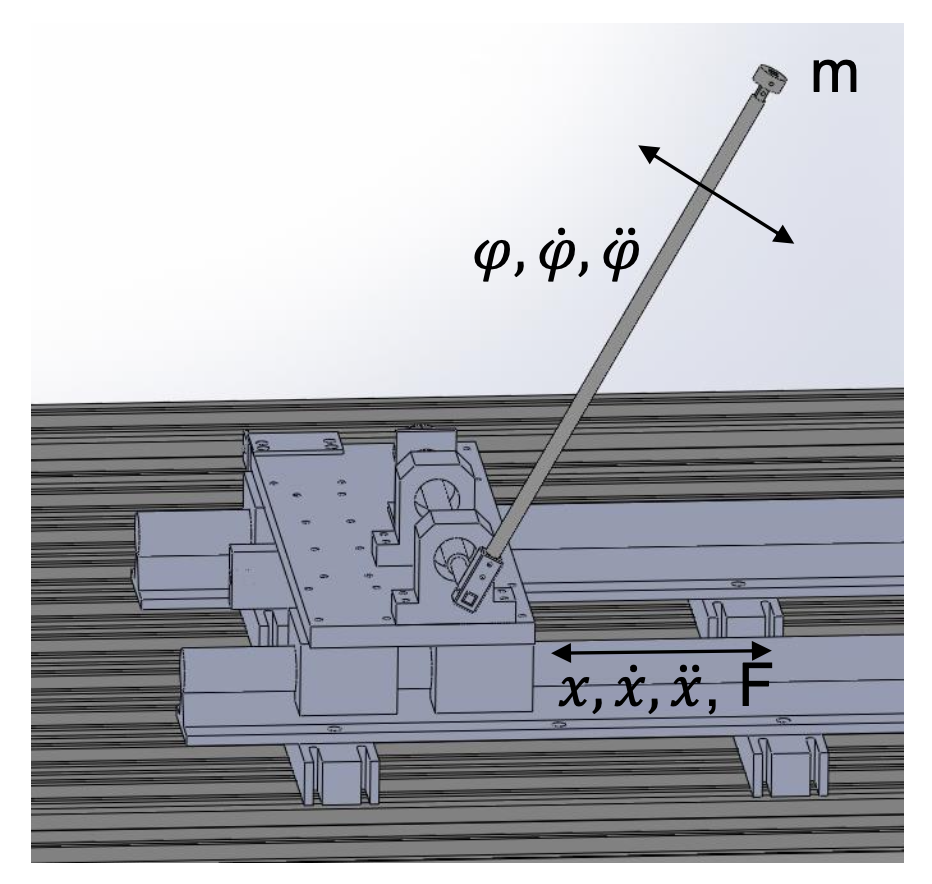
\includegraphics[width = 0.3\textwidth]{pendulum.png}
    \caption[Inverse pendulum sketch]{sketch of inverse pendulum (\cite[]{skependel})
    \label{fig:pendulum}} %label should over the caption and then to ref.
\end{figure}\\
A sensor mounted on the joint measures the angle of the pendulum, and the sensor data is sent 
to the controller for claculate until the angle \ensuremath{\phi} reaches vertical equilibrium, aka. 0°.

%%%%%%%%%%%%%%%%%%%%%%%%%%%%%%%%%%%%%%%%%%%%%%%%%%%%%%%%%%%%%%%%%%%%%%%%%%%%%%%%%%%%%%%%%%%%%%%%%%%%%%%%%%%%%%%%%%%%%%%%%%%%%%
\section{Hydraulic system}
\label{sec:Hydsys}
The hydraulic system is built by ifas. This system consists of a pump, a tank, 
a hydraulic cylinder, a capsule accumulator, and a 4/3 servo valve as its primary components. \\
A hydraulic cylinder, also known as a linear hydraulic motor, is powered by the                                                                                             
incompressible liquid hydraulic fluid compressed within the cylinder. 
By altering the pressure on both sides of the piston, the piston is pushed to move from 
side to side, therefore propelling the piston rod. Sketc.h will be showen form Fig \ref*{fig:hydcylinder}.\\
\begin{figure}[htbp]
  \centering
  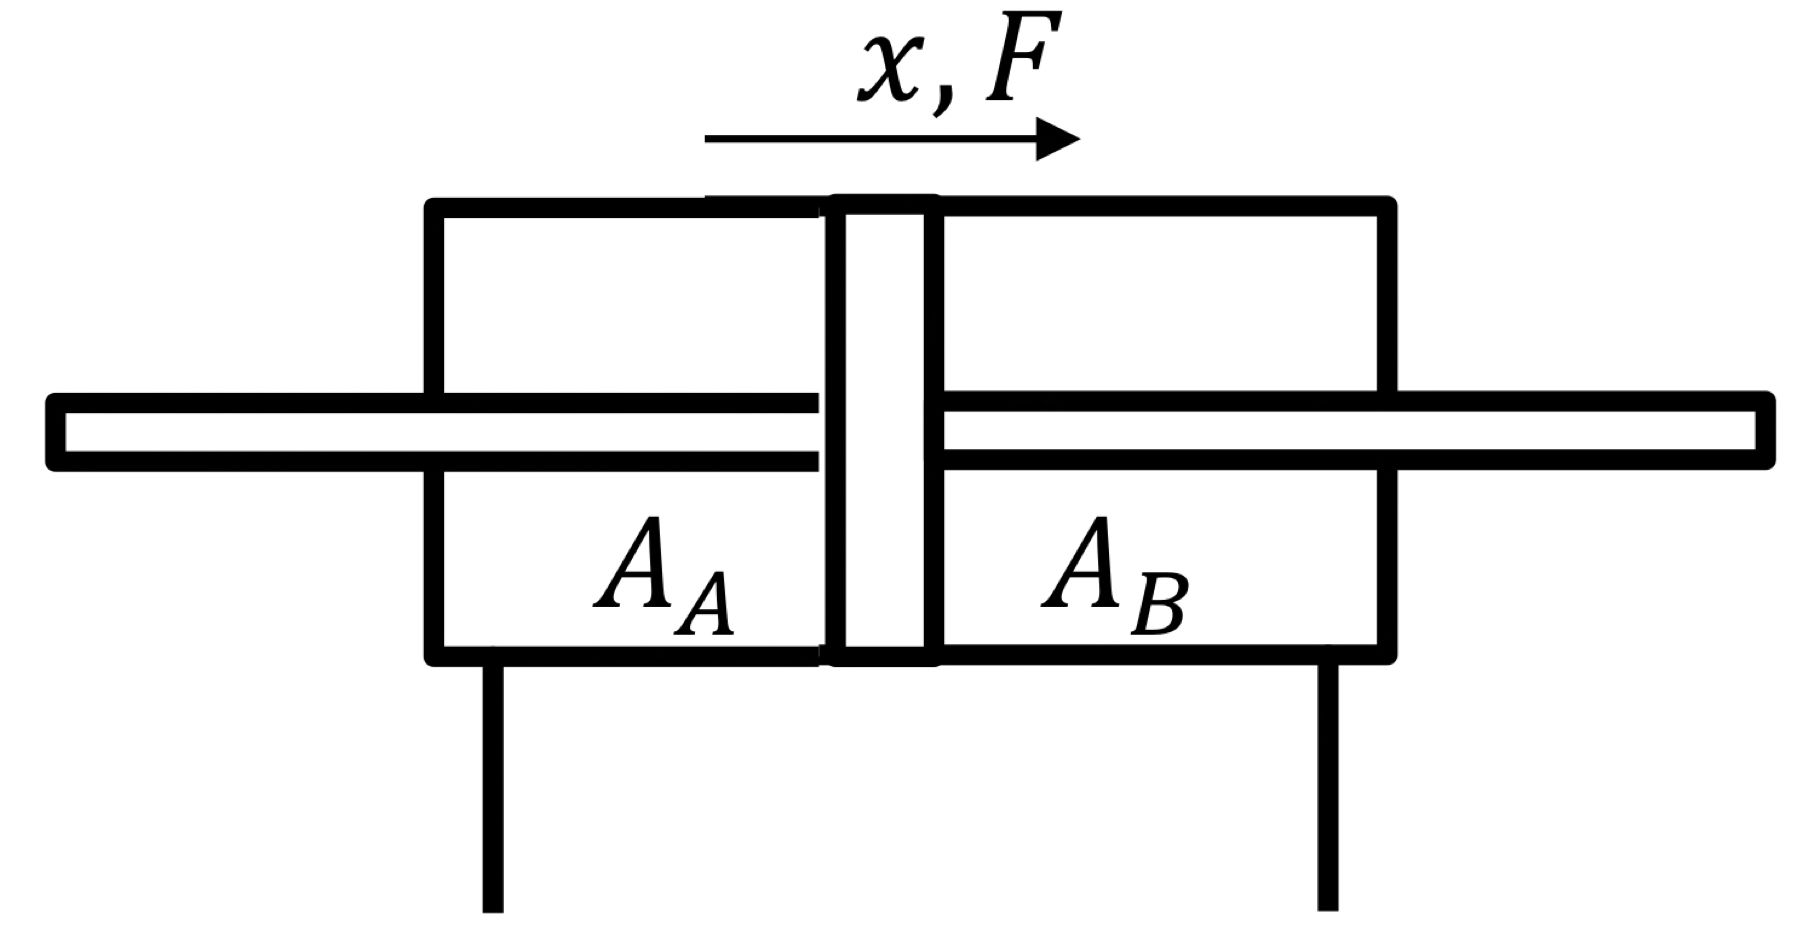
\includegraphics[width = 0.2\textwidth]{Contents/Resources/hydcylinder.jpeg}
  \caption[Hydraulic cylinder sketch]{Sketch of hydraulic cylinder}
  \label{fig:hydcylinder}
\end{figure}\\
Why would a hydraulic system be used to drive a cart instead of an electric motor? 
Hydraulics provides a simple yet effective method for generating a great deal of force 
in a small area, which was designed fairly early on and requires 
just a very tiny apparatus to raise 1 or 2 tons of objects with using the hydraulic force. 
Due to the incompressibility of hydraulic oil, the oil in the cylinder resembles a 
solid at high pressure, which gives the Hydraulic cylinder excellent dynamic properties.\\
\begin{figure}[htbp]
  \centering
  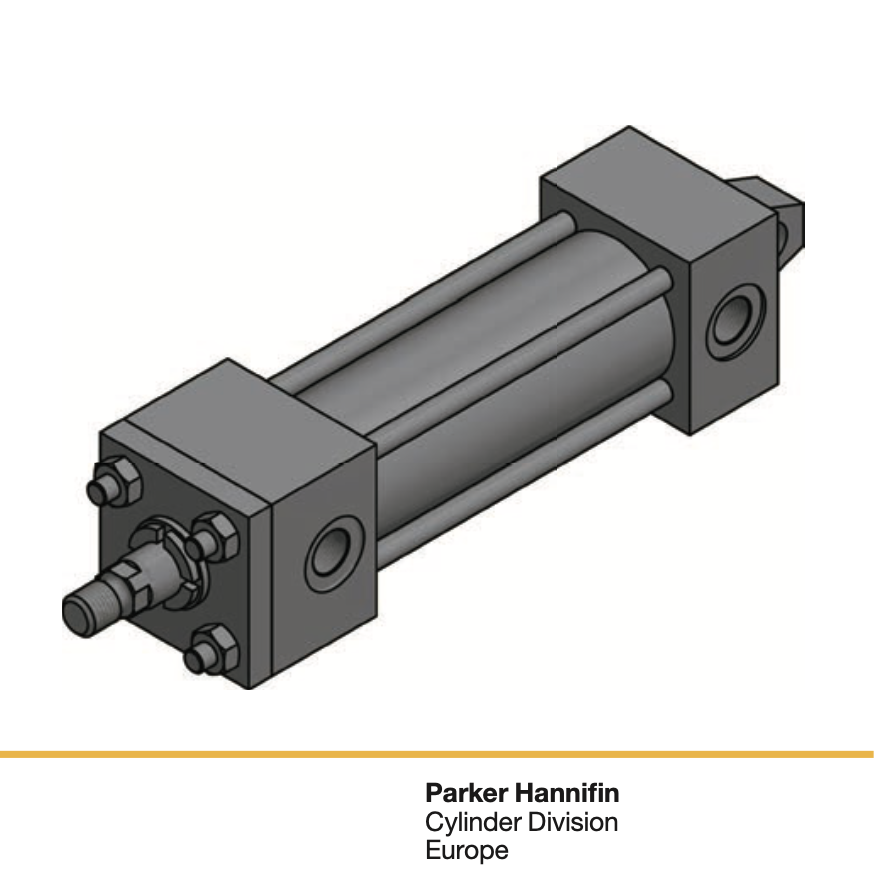
\includegraphics[width = 0.4\textwidth]{Contents/Resources/Parker Hydcylinder.png}
  \caption[Parker® Hydraulic cylinder]{Parker® hydraulic cylinder HMI-ME6(\cite[]{parker})}
  \label{fig:Parker}
\end{figure}\\
Existing hydraulic cylinder can provide working pressure up to 700bar. The hydraulic
cylinder in the unit is supplied by Parker® and the model HMI-ME6 can work up to 210 bar.

    \cleardoublepage

    \chapter{Description}
\label{ch:Description}
%%%%%%%%%%%%%%%%%%%%%%%%%%%%%%%%%%%%%%%%%%%%%%%%%%%%%%%%%%%%%%%%%%%%%%%%%%%%%%%%%%%%%%%%%%%%%%%%%%%%%%%%%%%%%%%%%%%%%%%%%%%%%%
\section{Description of system}


    \cleardoublepage

%   \include{Contents/98-Summary}
    \cleardoublepage



    \chapter{Outlook}
\label{ch:ausblick}
Hier kann man dann schreiben,was alles noch kommt.
    \cleardoublepage

    \chapter*{Beispielkapitel}  %with '*' will make the text be the subtext
\label{cha:beispielkapitel} %use \label{} to subscribe and the use \ref to chapt in 
Dieses Beispielkapitel dient der Darstellung häufig verwendeter Elemente in LaTeX wie Aufzählungen, Abbildungen, Tabellen oder Gleichungen. Es hat keinen Anspruch auf Vollständigkeit und kann gerne erweitert werden. Eine ausführliche Beschreibung der LaTeX-Befehle kann der Befehlsübersicht entnommen werden.
Die Beispiele können kopiert und dann angepasst werden.
% Abschnitt 1 --------------------------------------------------------------
% 		Name des Abschnittes
% --------------------------------------------------------------------------


\section*{Aufzählungen} %without '*' will get a subsection with number "3.1, 3.2"
\label{sec:aufzaehlungen}

\subsection*{Aufzählungen mit Punkten}
\label{aufzaehlung_punkte}

\begin{itemize}
    \item Körper
    \item Bindungselemente
    \item Koppelelemente
\end{itemize}

\subsection{Aufzählungen mit Zahlen} %without '*' will get a subsection with number "3.1.1, 3.1.2"
\label{aufzaehlung_zaheln}

\begin{enumerate}
    \item Körper
    \item Bindungselemente
    \item Koppelelemente
\end{enumerate}

\cleardoublepage
% Abschnitt 2 --------------------------------------------------------------
% 		Name des Abschnittes
% --------------------------------------------------------------------------


\section*{Abbildungen}
\label{sec:abbildungen}

\begin{figure}[htbp]
    \centering
    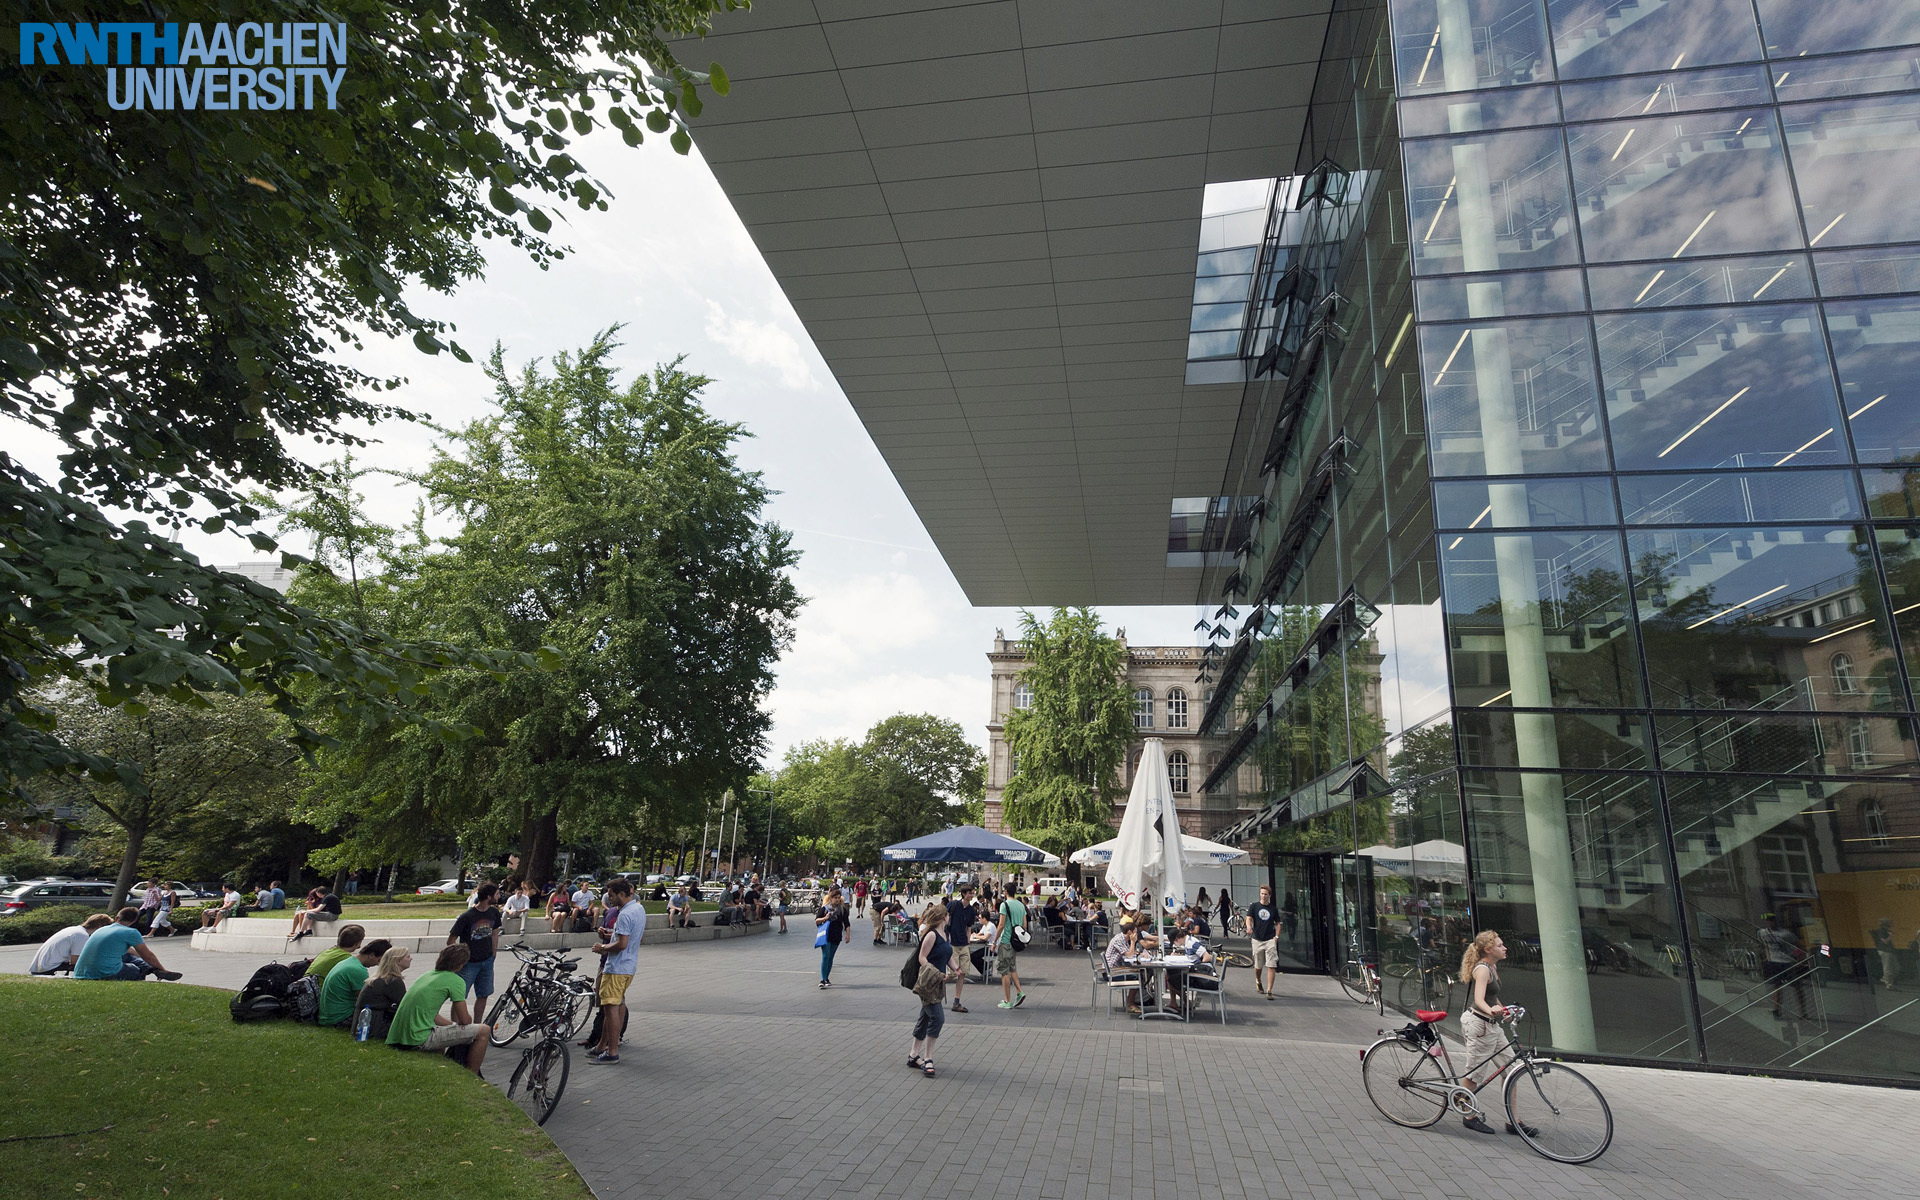
\includegraphics[width = 0.5\textwidth]{Contents/Resources/superc.jpeg}
    \caption[Eine Abbildung (kurze Abbildungsunterschrift ohne Quelle)]{Eine Abbildung (lange Abbildungsunterschrift mit Quelle, Quelle: \cite[1]{Mustermann.2012})}
    \label{fig:eine_abbildung}
\end{figure}

\begin{figure}[htbp]
    \centering
    \begin{subfigure}[t]{0.45\textwidth}
        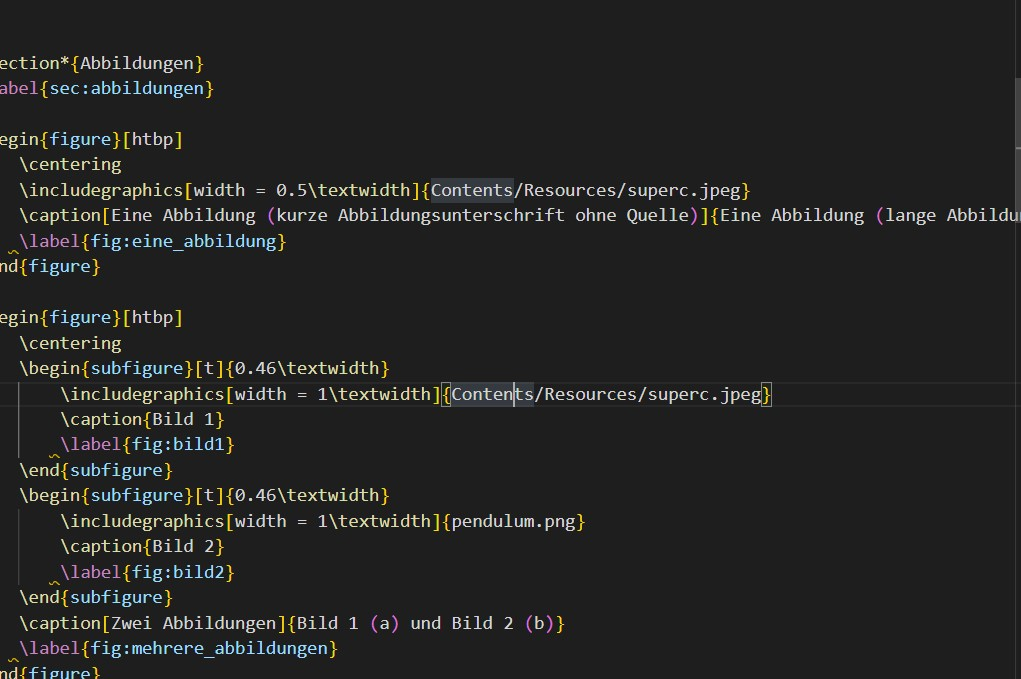
\includegraphics[width = 1\textwidth]{Contents/Resources/1103.jpg}
        \caption{Bild 1}
        \label{fig:bild1}
    \end{subfigure}
    \begin{subfigure}[t]{0.46\textwidth}
        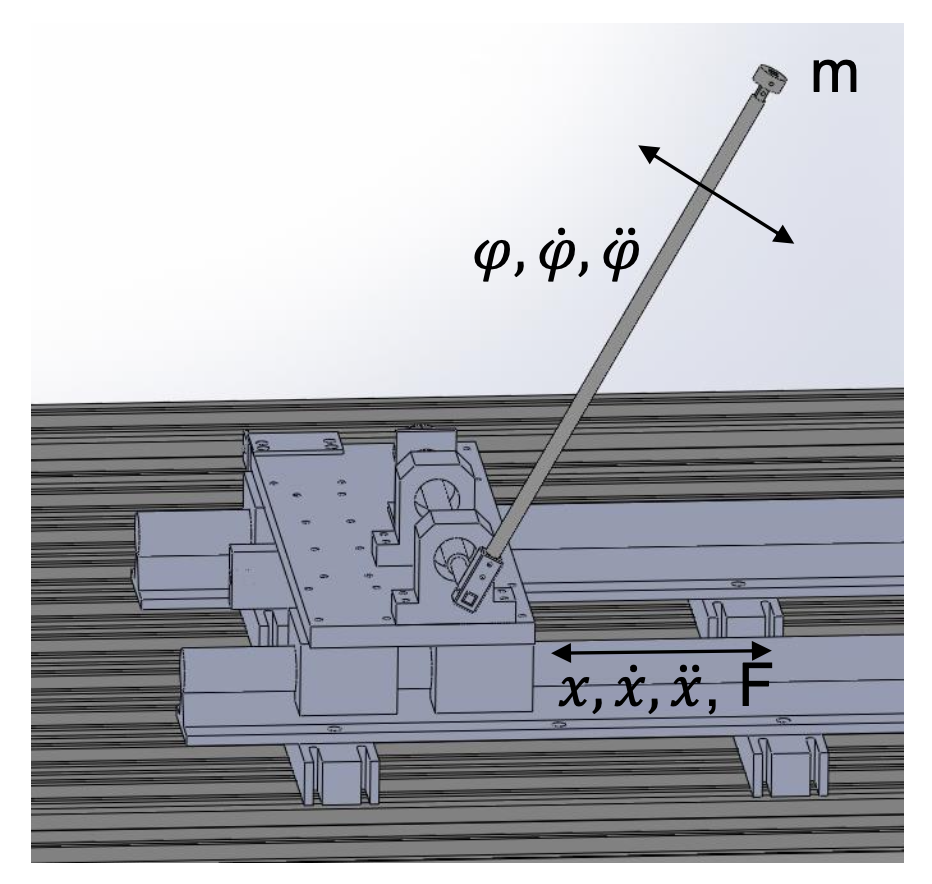
\includegraphics[width = 1\textwidth]{pendulum.png}
        \caption{Bild 2}
        \label{fig:bild2}
    \end{subfigure}
    \caption[Zwei Abbildungen]{Bild 1 (a) und Bild 2 (b)}
    \label{fig:mehrere_abbildungen}
\end{figure}

\cleardoublepage
% Abschnitt 3 --------------------------------------------------------------
% 		Name des Abschnittes
% --------------------------------------------------------------------------


\section*{Tabellen}
\label{sec:tabellen}

\begin{table}[htbp]
    \centering
    \caption{Tabelle mit automatischer Ausrichtung}
    \begin{tabular}{lcr}
        \toprule
        l & c   & r   \\
        \midrule
        a     & b   & c\\[0.25em]
        aa    & bb  & cc\\[0.25em]
        aaa   & bbb & ccc \\
        \bottomrule
    \end{tabular}
    \label{tab:tabelle1}
\end{table}

\begin{table}[htbp]
    \centering
    \caption{Tabelle mit Ausrichtung an Trennungszeichen}
    \begin{tabular}{R{4}{3} R{4}{0}}
        \toprule
        \multicolumn{1}{c}{a} & \multicolumn{1}{c}{b} \\
        \midrule
        1,234                & 1234                  \\
        12,34                & 123                   \\
        123,4                & 12                    \\
        1234                 & 1                     \\
    \end{tabular}
    \label{tab:tabelle2}
\end{table}

\begin{table}[htbp]
    \centering
    \caption{Tabelle mit Zellen über mehrere Zeilen oder Spalten}
    \begin{tabular}{lcr}
        \toprule
        l               & c   & r   \\
        \midrule
        \multicolumn{2}{c}{ab} & c\\[0.25em]
        \multirow{2}{*}{aa} & bb  & cc\\[0.25em]
        & bbb & ccc \\
        \bottomrule
    \end{tabular}
    \label{tab:tabelle3}
\end{table}

%\begin{table}[htbp]
%  \centering
%  \caption{Mehrere Untertabellen}
%  \subtable[Tabelle 1]{
%    \centering  
%\begin{tabular}{lcr}
%	 	\toprule
%	 	l & c & r\\
%	 	\midrule
%		a & b & c\\[0.25em]
%		aa & bb & cc\\[0.25em]
%		aaa & bbb & ccc\\
%		\bottomrule
%	\end{tabular}	
%  }
%  \subtable[Tabelle 2]{
%    \centering  
%\begin{tabular}{lcr}
%	 	\toprule
%	 	l & c & r\\
%	 	\midrule
%		a & b & c\\[0.25em]
%		aa & bb & cc\\[0.25em]
%		aaa & bbb & ccc\\
%		\bottomrule
%	\end{tabular}	
%  }
%\label{tab:tabellen}
%\end{table}

\cleardoublepage
% Abschnitt 4 --------------------------------------------------------------
% 		Name des Abschnittes
% --------------------------------------------------------------------------


\section*{Gleichungen}
\label{sec:gleichungen}

Newton hat folgenden Zusammenhang entdeckt:
\begin{align}
    F = m a
    \label{eqn:newton}
\end{align}
Das war das mit dem Apfel und so.

\section*{Anführungszeichen}
\label{sec:anfuehrungszeichen}
Es gibt mehrere Möglichkeiten deutsche Anführungszeichen einzufügen:\\
\glqq test\grqq\\
"`test"'\\


\section*{Zitationen}

Zitation einer Quelle: \cite{Mustermann.2012}\\
Zitation einer Quelle mit Seitenangabe: \cite[12-16]{Mustermann.2012}\\
Zitation mehrerer Quellen: \cites{Mustermann.2012}{Musterfrau.2011}\\
Zitation mehrerer Quellen mit Seitenangabe: \cites[12-16]{Mustermann.2012}[3]{Musterfrau.2011}\\


    \cleardoublepage

    \pagenumbering{Roman}
% --------------------------------------------------------------------------
%		Literaturverzeichnis / List of literature
% --------------------------------------------------------------------------
    \printbibliography[heading=bibintoc,title=List of literature]

% --------------------------------------------------------------------------
%		Tabellenverzeichnis / List of tables
% --------------------------------------------------------------------------
    \listoftables                        % Tabellenverzeichnis / List of tables
    \cleardoublepage

% --------------------------------------------------------------------------
%		Abbildungsverzeichnis / Register of illustrations
% --------------------------------------------------------------------------
    \listoffigures                        % Abbildungsverzeichnis / Register of illustrations
    \cleardoublepage

% --------------------------------------------------------------------------
%		Anhang / Attachment
%
%		Der Anhnag enthält weitere Dokumente, welche nicht direkt zur Arbeit
%		gehören oder aus Platzgründen ausgelagert werden müssen. Die Kapitel
%		des Anhangs werden mit Großbuchstaben bezeichnet
%
%		The attachment contains further documents which are not related to work directly or
%		had to be outsourced due to a lack of space. The different chapters of the attachment
%		are labeled with a captital letter.
% --------------------------------------------------------------------------
    \appendix

% Inhalt des Anhangs (Beispiel) / List of contents of attachment (Example)
%    SPJ: Ich habe keinen Anhang
%    \chapter{Figure}
\label{ch:anhang_abbildungen}

%    \cleardoublepage
%    \chapter{Tabellen}
\label{ch:anhang_tabellen}

% TODO: Paket longtable ??
% https://www.till-biskup.de/_media/de/lehre/latex/ss2018/05/kurs-latex-05.pdf (Folie 32)

\input{Contents/Attachment/PI-Table}
%    \cleardoublepage

    \backmatter
\end{document}
